The advanced usage of CUP in this chapter includes:
\begin{itemize}
    \item
    grammars with ambiguities;
    \item
    lists;
    \item
    operator precedence;
    \item
    handling syntax errors.
\end{itemize}

\section{Ambiguous Grammars in CUP}
Conflicts can arise when the grammar is ambiguous; this implies that the parser must choose between two or more alternative actions.
The problem can be resolved by modifying the grammar (in order to make it non-ambiguous) or by instructing the parser on how to handle ambiguity.
The latter option requires that the parsing algorithm is fully understood, in order to avoid unwanted/wrong behaviors.

A grammar is ambiguous if there is at least one sequence of symbols for which two or more distinct parse trees exist.

Example:
\begin{lstlisting}
S ::= M;
M ::= 'if' C M;
M ::= 'if' C M 'else' M;
M ::= ID '=' NUM ';'
    | ID '=' ID ';';
C ::= '(' VAR '==' NUM ';';
\end{lstlisting}
This grammar is ambiguous; it is possible to convert it to this way:
\begin{lstlisting}
S ::= M
    | U;
U ::= 'if' C S;
U ::= 'if' C M 'else' U;
M ::= 'if' C M 'else' M;
M ::= ID '=' NUM ';'
    | ID ';';
C ::= '(' ID '==' NUM ')';
\end{lstlisting}

\subsection{Non-Ambiguous Grammar Example: Algebraic Expressions}
The non-ambiguous grammar that describes an algebraic expression is the following:
\begin{lstlisting}
S ::= E
E ::= E '+' T
E ::= E '-' T
E ::= T
T ::= T '*' F
T ::= T '/' F
T ::= F
F ::= '(' E ')'
F ::= NUM
\end{lstlisting}
The symbols \code{T} and \code{F} are used to solve the ambiguity given by the priority of operators ``\code{+}'' and ``\code{-}''.

\subsection{Ambiguous Grammar in CUP}
\subsubsection{Example of Shift-Reduce Conflicts}
Rules:
\begin{enumerate}
    \item
    \code{S :: = 'if' E 'then' S}
    \item
    \code{S :: = 'if' E 'then' S 'else' S}
    \item
    \code{S :: = V}
\end{enumerate}
The input is the following:
\begin{lstlisting}[mathescape]
if E then if E then V $\bullet$ else V
\end{lstlisting}

Stack situation:
\begin{figure}[H]
    \centerline{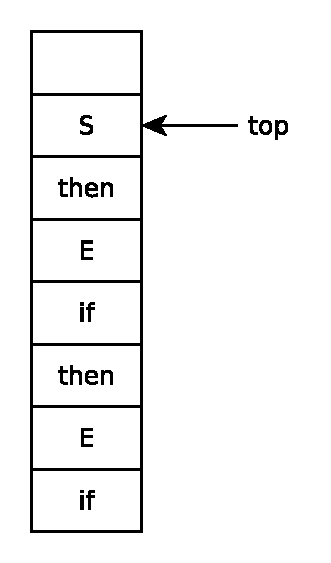
\includegraphics[width=0.2\textwidth]{img/20.pdf}}
\end{figure}

Possible actions:
\begin{enumerate}
    \item
    shift \code{else} token into the stack (rule 2);
    \begin{figure}[H]
        \centerline{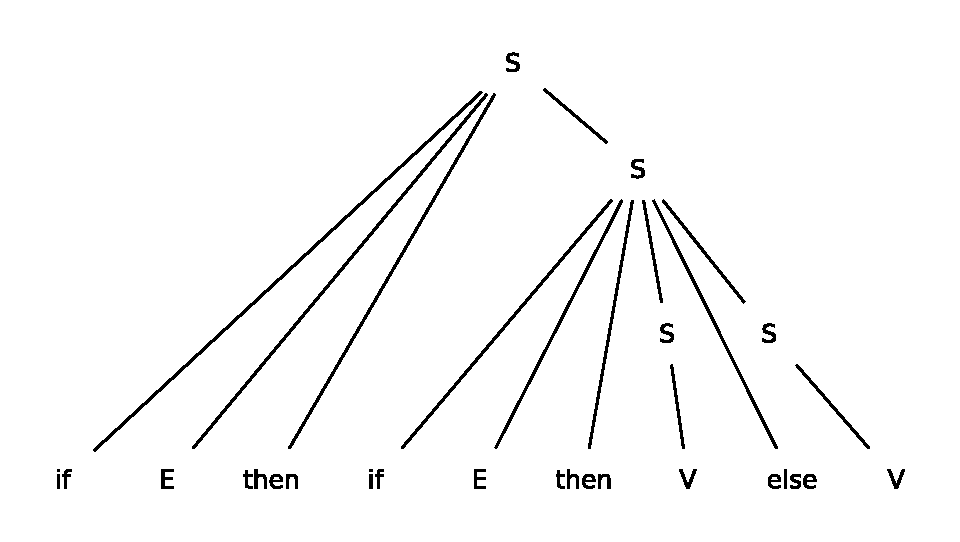
\includegraphics[width=0.6\textwidth]{img/21.pdf}}
    \end{figure}
    \item
    reduce the first four top elements of the stack (rule 1);
    \begin{figure}[H]
        \centerline{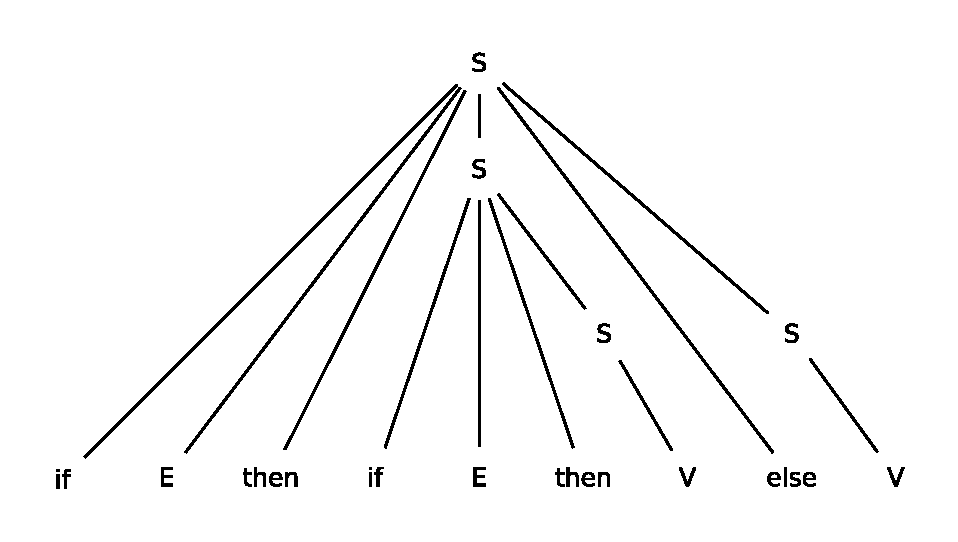
\includegraphics[width=0.6\textwidth]{img/22.pdf}}
    \end{figure}
\end{enumerate}

A possible solution is that CUP performs a Shift action and then the resulting parse tree is the following:
\begin{figure}[H]
    \centerline{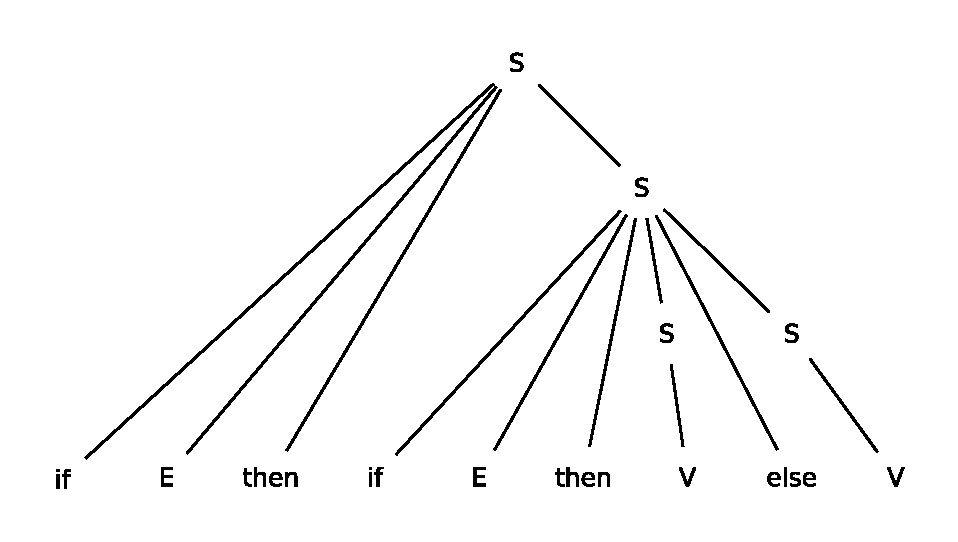
\includegraphics[width=0.6\textwidth]{img/23.pdf}}
\end{figure}

\subsubsection{Example of Reduce-Reduce Conflict}
Rules:
\begin{enumerate}
    \item
    \code{S :: = a B}
    \item
    \code{S :: = B}
    \item
    \code{S :: = a b}
    \item
    \code{S :: = b}
\end{enumerate}
The input is the following:
\begin{lstlisting}[mathescape]
a b
\end{lstlisting}
The next token is \code{EOF}.

Stack situation:
\begin{figure}[H]
    \centerline{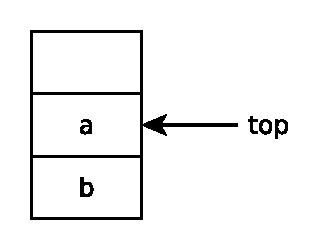
\includegraphics[width=0.2\textwidth]{img/24.pdf}}
\end{figure}
Two possible actions:
\begin{enumerate}
    \item
    reduce the first two top elements of the stack (rule 3);
    \begin{figure}[H]
        \centerline{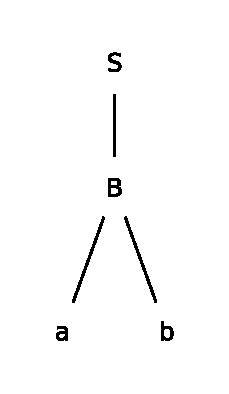
\includegraphics[width=0.6\textwidth]{img/25.pdf}}
    \end{figure}
    \item
    reduce the first top element of the stack (rule 4);
    \begin{figure}[H]
        \centerline{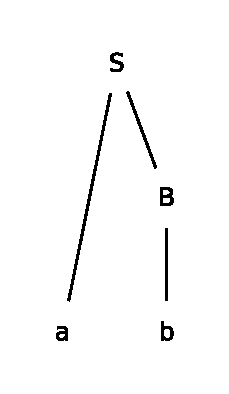
\includegraphics[width=0.6\textwidth]{img/26.pdf}}
    \end{figure}
\end{enumerate}
CUP can perform a reduction using the first defined rule (rule 3)\footnote{Simply because of rule order: rule 3 comes first than rule 4.}.

\section{Lists}
\subsubsection{Examples with Lists}

\section{Precedence Section: Ambiguous Grammars}

\section{Associativity}

\section{Precedence Section: Operators}

\section{User Code}

\subsubsection{Errors-Printing Line and Column}

\section{Handling Syntax Errors}

\subsection{\code{ERROR} Predefined Symbol}

\section{Attributes of Symbols}

\section{Synthesized Attributes}

